\chapter{Implementación}

La implementación del software se ha dividido en hitos. Estos han sido definidos en GitHub
y cada uno de ellos contiene un grupo de \textit{issues} que se corresponden con las distintas
mejoras que se han ido incorporando al software a lo largo de su desarrollo.

Cada milestone representa un bloque de trabajo con un objetivo definido, lo que permite seguir
un enfoque ágil, enfocado en construir progresivamente un prototipo sólido en lugar de intentar
desarrollar todo el sistema de una vez. 

\section{Milestone 1: Elección del lenguaje de programación}
En este primer hito se decidió el lenguaje de programación a utilizar para el desarrollo del software,
siendo Python la opción elegida. Esta elección se justificó y documentó debidamente en el
\hyperref[sec:lenguaje-programación]{anterior capítulo}.

\section{Milestone 2: Modelo del problema}
Este hito se centra en dos tareas principales: la configuración de las herramientas necesarias para
el desarrollo guiado por pruebas, y la definición del modelo del dominio siguiendo el enfoque 
\textit{Domain-Driven Design} (DDD).

\subsection{Configuración del entorno de desarrollo}
En el capítulo anterior se seleccionaron las herramientas que se emplearían para 
\hyperref[sec:gestor-dependencias]{gestionar las dependencias y el entorno} y 
\hyperref[sec:herramienta-testeo]{realizar pruebas}. En este hito se procedió a su instalación y 
configuración.

\subsubsection{Poetry}
Se ha usado \textit{Poetry} para gestionar las dependencias y el entorno virtual del proyecto.

Al inicializar el gestor, se genera automáticamente un archivo \texttt{pyproject.toml} en la raíz del
repositorio, que contiene la información básica del proyecto y servirá como punto central
para la gestión de dependencias.

\subsubsection{Pytest}
La herramienta seleccionada para las pruebas unitarias ha sido \texttt{pytest}.
La elección de esta herramienta ya fue justificada en el capítulo anterior.

Se ha añadido \texttt{pytest} como dependencia, lo que significa que se instalará únicamente
para el entorno de desarrollo y no se considera una dependencia necesaria para la ejecución del 
prototipo en producción. De esta manera se mantiene una separación clara entre las librerías 
empleadas para programar y probar el software, y aquellas que serán estrictamente necesarias para 
su despliegue.

Al instalar dependencias mediante Poetry, junto al archivo \texttt{pyproject.toml} se genera 
automáticamente el archivo \texttt{poetry.lock}. El primero declara qué dependencias se requieren y 
en qué rango de versiones son aceptables; en cambio, el archivo \texttt{poetry.lock} registra la 
versión exacta de esas dependencias en el momento de la instalación. Gracias a este mecanismo se 
garantiza la reproducibilidad del entorno, ya que cualquier persona que clone el repositorio e 
instale las dependencias obtendrá exactamente las mismas versiones usadas en el desarrollo 
original.

\subsection{Modelo del dominio}
El modelado del dominio se ha realizado siguiendo el enfoque \textit{Domain-Driven Design} (DDD)
propuesto por Eric Evans \cite{evansDDD}. Este método de diseño de software se centra en que
el sistema refleje fielmente la realidad del dominio que se está modelando, evitando que los 
aspectos técnicos o de implementación condicionen la representación del problema.

Uno de los principios fundamentales de DDD es la creación de un \textit{lenguaje ubicuo}, introducido
por Evans en el capítulo 2 de su obra \cite{evansDDD}. Esto consiste en definir términos y conceptos 
específicos del dominio para que los conceptos empleados en el código coincidan con los del propio 
dominio. De este modo se facilita la comunicación entre el análisis y la implementación. En este 
proyecto se ha definido el siguiente lenguaje ubicuo:

\begin{itemize}
    \item \textbf{Escudo}: Entendemos como escudo a la representación gráfica de un conjunto de
    elementos heráldicos que identifican a una persona, entidad o institución.
    \item \textbf{Blasón}: Descripción textual del escudo.
    \item \textbf{Portador}: Persona, entidad o institución a la que pertenece el escudo.
    \item \textbf{Campo}: Superficie del escudo donde se disponen los elementos heráldicos.
    \item \textbf{Boca}: Forma exterior del escudo, es decir, su contorno.
    \item \textbf{Partición}: Cada una de las divisiones del campo del escudo. 
    \item \textbf{Esmalte}: Color o metal con el que se pinta un elemento heráldico.
    \begin{figure}[H]
        \centering
        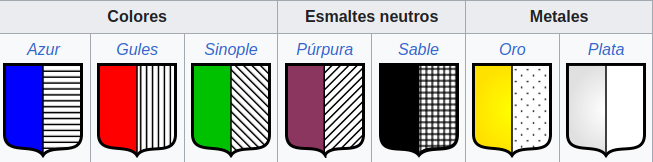
\includegraphics[width=0.7\textwidth]{figuras/esmaltes-canonicos.png}
        \caption{Esmaltes heráldicos canónicos. Imagen de dominio público, Wikimedia Commons.}
        \label{fig:esmaltes}
    \end{figure}
    \item \textbf{Pieza heráldica}: Son elementos de distinto esmalte al del campo que suelen tocar
    los bordes del escudo.
    \item \textbf{Figura o mueble}: Son todo aquello que se encuentra dentro del campo del escudo y
    no resulta ser una pieza heráldica.
    \item \textbf{Adorno exterior}: Son todos aquellos elementos que no se encuentran dentro del campo
    del escudo.
\end{itemize}

\begin{figure}[H]
    \centering
    
\includegraphics[width=1\textwidth]{figuras/escudo-papa-francisco.png}
    \caption{Partes del escudo de armas del papa Francisco \cite{wikiEscudo}.}
    \label{fig:partes-escudo}
\end{figure}

Las definiciones empleadas en este lenguaje ubicuo se han extraído del 
\textit{Manual de heráldica: la ciencia del blasón} \cite{delgadoHeraldica}.

En esta primera iteración se ha decidido limitar el modelo a una parte reducida del lenguaje ubicuo. 
Concretamente, se trabajará con el \textbf{Escudo} como composición de otros elementos, incorporando 
inicialmente el \textbf{Campo} y el \textbf{Esmalte}, que constituyen la base mínima necesaria para 
definir un prototipo funcional. 

Otros elementos como la \textbf{Boca}, el \textbf{Portador}, las \textbf{Particiones}, las 
\textbf{Piezas heráldicas}, las \textbf{Figuras} o los \textbf{Adornos exteriores} se han recogido 
en el lenguaje ubicuo, pero quedan fuera del alcance de esta iteración y se abordarán en futuras 
extensiones del modelo.

\subsection{Desarrollo dirigido por pruebas (TDD)}

El modelo inicial del dominio se ha implementado siguiendo la metodología de 
\textit{Test-Driven Development} (TDD) \cite{beckTDD}. Esto significa que antes de escribir 
el código se definieron las pruebas que debía superar, y después se implementó lo mínimo necesario 
para que pasaran.

En esta primera iteración se definieron pruebas unitarias para los elementos básicos 
del modelo: \texttt{Esmalte}, \texttt{Campo} y \texttt{Escudo}. Dichas pruebas validan:

\begin{itemize}
    \item Que un \texttt{Escudo} válido puede crearse a partir de un \texttt{Campo} 
    con un \texttt{Esmalte} permitido.
    \item Que los intentos de producir un \texttt{Esmalte} con valores no reconocidos producen 
    una excepción.
    \item Que no es posible instanciar un \texttt{Campo} sin un \texttt{Esmalte} válido.
\end{itemize}

Al principio estas pruebas no pasan, ya que no existe ninguna implementación. A continuación se
escribe el código mínimo necesario para que todas las pruebas definidas pasen correctamente. Esto
se repetirá cada vez que se añada una nueva funcionalidad al modelo.

Como resultado surgieron las clases \texttt{Esmalte}, \texttt{Campo} y \texttt{Escudo}, que constituyen 
la base mínima del dominio:

\begin{itemize}
    \item \texttt{Esmalte}: representa los colores y metales permitidos en heráldica. 
    Comprueba que el valor introducido sea válido y lo normaliza.
    \item \texttt{Campo}: representa la superficie del escudo. Solo puede generarse 
    si se le proporciona un \texttt{Esmalte} válido.
    \item \texttt{Escudo}: actúa como elemento principal y se compone de un \texttt{Campo}.
\end{itemize}

\section{Milestone 3: Identificación y filtrado por esmalte}

En este milestone se introduce la primera lógica de negocio, que consiste en filtrar los escudos
por el esmalte del campo. Esto facilita la identificación de escudos de \hyperref[sec:hu1]{HU1} y 
la clasificación y el filtrado de escudos de \hyperref[sec:hu2]{HU2}.

Para ello, es necesario implementar un catálogo mínimo de ejemplo para poder realizar la consulta.

Los criterios de aceptación son sencillos: (1) dado un esmalte válido, la consulta devuelve 
únicamente escudos con ese campo; (2) sin criterio, se devuelve el catálogo completo; y 
(3) con un criterio erróneo, la respuesta es una lista vacía.

\subsection{Adición de un catálogo mínimo}

En este punto no había ningún escudo cargado y, por tanto, no había nada que filtrar. Antes 
de implementar la búsqueda por esmalte del campo, lo razonable era añadir al sistema un catálogo 
base sobre el que poder trabajar y comprobar el comportamiento.

Para este hito opté por un catálogo mínimo y en memoria, dentro del propio paquete. 
Cada entrada se modela como una pequeña ficha con el nombre del escudo y el esmalte.
El campo se guarda como un Esmalte, de modo que queda validado y normalizado desde
el minuto uno y se evitan incoherencias.

Se han añadido a este catálogo siete escudos, uno para cada esmalte canónico, con la finalidad de
poder probar la búsqueda de cualquier esmalte. La decisión de mantener el catálogo en memoria
simplifica la implementación inicial y permite centrarse en la funcionalidad de filtrado sin
introducir complejidades adicionales que se tratarán en futuros hitos, como la implementación
de una base de datos.

Siguiendo TDD, primero escribí unas pruebas muy básicas: que el catálogo no esté vacío y que el 
campo de cada ficha sea un Esmalte. Con esas pruebas en rojo implementé lo mínimo para ponerlas en
verde: un catálogo pequeño en memoria y la función listar(). Con eso ya está lista la base para el
siguiente paso: filtrar la búsqueda por el esmalte del campo.

\subsection{Búsqueda por esmalte del campo}
Para satisfacer la necesidad de identificar y filtrar rápidamente escudos a partir de un rasgo visual
inmediato, se implementa la búsqueda por esmalte del campo. Esta funcionalidad cubre lo definido en la
\hyperref[sec:hu1]{HU1}: permite localizar los escudos cuyo campo presenta un esmalte determinado, y
resolverá eventualmente la \hyperref[sec:hu2]{HU2}, al facilitar la clasificación y el filtrado de escudos.

Siguiendo la metodología TDD, primero escribí las pruebas unitarias que definen los criterios de
aceptación de esta funcionalidad:

\begin{itemize}
    \item Dado un \hyperref[fig:esmaltes]{esmalte canónico}, la consulta devuelve únicamente escudos con ese campo.
    \item Sin criterio, se devuelve el catálogo completo.
    \item Con un criterio no canónico, la respuesta es una lista vacía.
\end{itemize}

Después implementé la función de filtrado para poner esos tests en verde. La validación, así como 
la normalización del criterio, se delega en \texttt{Esmalte}, de forma que la lógica de
búsqueda se mantiene simple.

\subsection{Normalización del esmalte}
Para que la búsqueda por esmalte sea más amigable y no requiera que el usuario conozca los términos
heráldicos exactos, se ha añadido un mecanismo de normalización en la clase \texttt{Esmalte}. 
Este mecanismo mapea términos coloquiales a sus equivalentes heráldicos canónicos. Por ejemplo,
``rojo'' se mapea a ``gules'' y ``azul'' a ``azur''. De este modo, si el usuario introduce un término común,
el sistema lo normaliza automáticamente, facilitando la búsqueda.

\section{Milestone 4: Ampliación del catálogo y mejoras en el filtrado}
En el modelado inicial realizado en el M2 se limitó el dominio de los escudos a los elementos más 
básicos: ``campo'' y ``esmalte''. Esta representación mínima permitía trabajar con un prototipo funcional, 
pero restringía la capacidad de hacer búsquedas más complejas o de analizar atributos adicionales 
de los escudos.

En esta nueva iteración (M4), se amplía el modelo para incluir un subconjunto representativo de 
componentes adicionales, con el objetivo de habilitar búsquedas más avanzadas y preparar la estructura 
para futuras integraciones.

Los nuevos elementos incorporados al modelo son: 

\begin{itemize}
    \item \textbf{Pieza heráldica}: Se representa como un segundo esmalte, aplicando la regla heráldica
    de no poner metal sobre metal ni color sobre color. Esto permite buscar por color sin necesidad de
    saber cuál es el esmalte del campo y cuál el de la pieza. En futuras iteraciones se podría ampliar
    este concepto para incluir la forma de la pieza.
    \item \textbf{Adorno exterior}: Se representa como un subconjunto de elementos seleccionados de la
    heráldica real, como la corona, el yelmo o la mitra, entre otros. Cada adorno puede estar asociado
    a una categoría interna (papal, episcopal y noble) para además de poder filtrar por adorno, se pueda
    filtrar por categoría. Se permite que un escudo tenga cero o más adornos. Este conjunto puede ampliarse
    en futuras iteraciones.

    \begin{figure}[h!]
    \centering

    \begin{minipage}{0.3\textwidth}
        \centering
        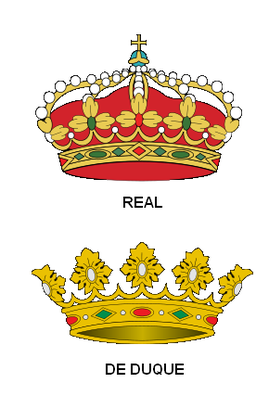
\includegraphics[width=\textwidth]{figuras/coronas.png}
        \caption{Coronas heráldicas seleccionadas. Imagen de dominio público, Wikimedia Commons.}
    \end{minipage}
    \hfill
    \begin{minipage}{0.3\textwidth}
        \centering
        
\includegraphics[width=\textwidth]{figuras/mitra.png}
        \caption{Mitra heráldica seleccionada. Imagen de Xavigivax, Wikimedia Commons, CC BY-SA 4.0.}
    \end{minipage}
    \hfill
    \begin{minipage}{0.3\textwidth}
        \centering
        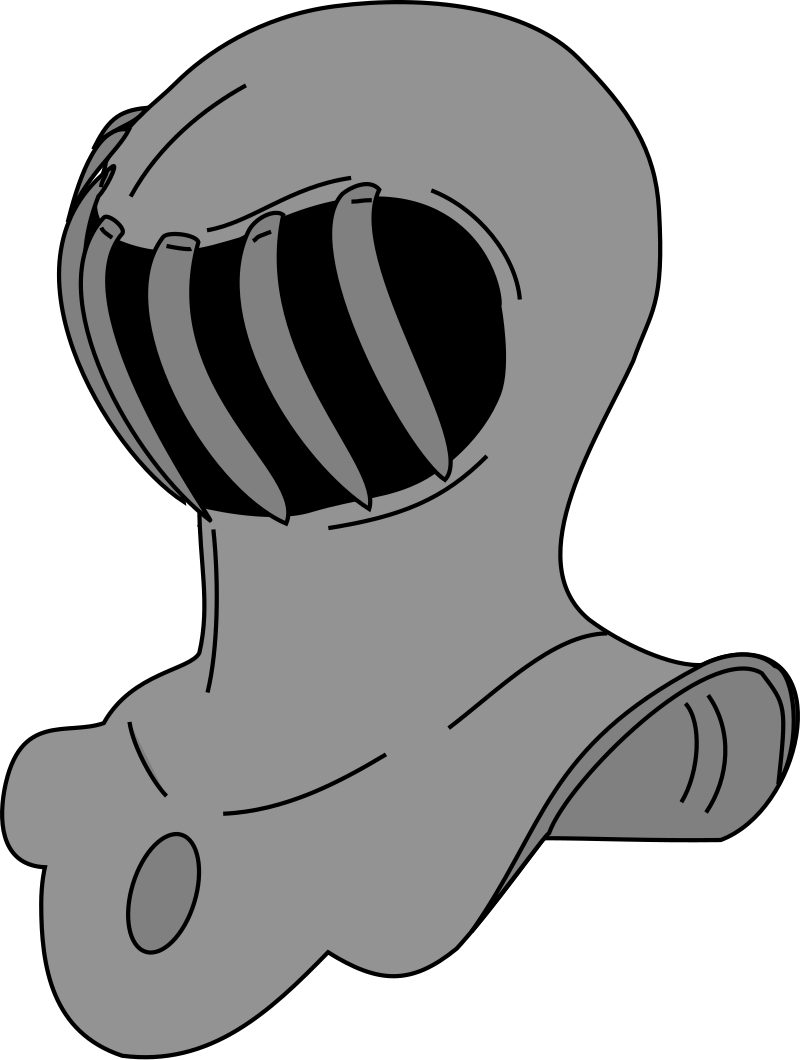
\includegraphics[width=\textwidth]{figuras/yelmo.png}
        \caption{Yelmo heráldico seleccionado. Imagen de Zigeuner, Wikimedia Commons, CC BY-SA 3.0.}
    \end{minipage}

    \caption{Adornos exteriores representativos en heráldica.}
    \label{fig:adornos_exteriores}
\end{figure}


    \item \textbf{Portador}: Se añade el portador como un atributo obligatorio del escudo, representado
    como un string normalizado (sin minúsculas, tildes ni espacios). Esto permite identificar a quién 
    pertenece el escudo y facilita búsquedas basadas en el portador.
    \item \textbf{Mueble}: Se representa como un subconjunto limitado de figuras heráldicas comunes,
    como el león, el castillo o la estrella. Cada escudo puede tener cero o más muebles, lo que facilita
    las búsquedas. Este conjunto podrá ampliarse en futuras iteraciones.

    \begin{figure}[h!]
        \centering

        \begin{minipage}{0.45\textwidth}
            \centering
            
\includegraphics[width=0.6\textwidth]{figuras/leon.png}
            \caption{León heráldico seleccionado. Imagen de VARGUX, Wikimedia Commons, CC BY-SA 4.0.}
        \end{minipage}
        \hfill
        \begin{minipage}{0.45\textwidth}
            \centering
            
\includegraphics[width=0.6\textwidth]{figuras/castillo.png}
            \caption{Castillo heráldico seleccionado. Imagen de Xavigivax, Wikimedia Commons, CC BY-SA 3.0.}
        \end{minipage}
    \end{figure}
\end{itemize}

Estos elementos se han seleccionado para proporcionar una base sólida que permita 
realizar búsquedas más detalladas y específicas, sin complicar excesivamente el modelo.

Siguiendo TDD, primero se definieron las pruebas unitarias que validan la correcta creación de estos 
nuevos elementos, las cuales consisten en:

\begin{itemize}
    \item \textbf{Pieza heráldica}: Validar que la pieza se crea correctamente con un esmalte válido y que
    se aplica la regla de no poner metal sobre metal ni color sobre color.
    \item \textbf{Adorno exterior}: Validar que únicamente se pueden añadir adornos del conjunto predefinido
    y que la categoría se asigna correctamente.
    \item \textbf{Portador}: Validar que el portador se normaliza correctamente y que es un atributo obligatorio.
    \item \textbf{Mueble}: Validar que únicamente se pueden añadir muebles del conjunto predefinido.
\end{itemize}

Posteriormente, se implementaron las clases de dominio y las modificaciones necesarias en los archivos 
de datos JSON. Esta aproximación permite que los tests unitarios pasen correctamente, garantizando la 
integridad de los escudos y preparando el sistema para futuras ampliaciones.

\subsection{Mejoras en el filtrado}
Con la ampliación del modelo, se han añadido nuevas funcionalidades de filtrado para aprovechar los
nuevos atributos. Ahora es posible filtrar escudos no solo por el esmalte del campo, sino también por
``portador'', ``pieza heráldica'', ``mueble'' y ``adorno exterior'', además de la categoría a la que
pertenece el escudo según su adorno exterior. Esto permite realizar búsquedas más específicas y detalladas,
facilitando la identificación de escudos.

Siguiendo la metodología TDD, se definieron pruebas unitarias para cada nuevo criterio de filtrado,
asegurando que cada uno funcione correctamente y que las combinaciones de filtros produzcan los
resultados esperados. Estas pruebas incluyen:
\begin{itemize}
    \item \textbf{Filtrado por ``portador''}: Validar que la búsqueda devuelve escudos cuyo portador coincide
        con el criterio proporcionado.
    \item \textbf{Filtrado por ``pieza heráldica''}: Validar que la búsqueda devuelve escudos que contienen
        la pieza heráldica especificada.
    \item \textbf{Filtrado por ``mueble''}: Validar que la búsqueda devuelve escudos que contienen el mueble
        especificado.
    \item \textbf{Filtrado por ``adorno exterior''}: Validar que la búsqueda devuelve escudos que incluyen
        el adorno exterior especificado.
    \item \textbf{Filtrado por ``categoría''}: Validar que la búsqueda devuelve escudos cuya categoría de
        adorno exterior coincide con el criterio proporcionado.
\end{itemize}

Para ello primeramente se actualizó el catálogo mínimo con escudos que incluyeran
estos nuevos atributos, y después se implementó la lógica de filtrado necesaria para que todas las
pruebas pasaran correctamente.

\section{Milestone 5: Creación de base de datos}
En este hito se sustituye el almacenamiento en JSON por una base de datos relacional que refleja el modelo actual. 
Este cambio permite persistir los datos de forma estable, mantener las relaciones entre los elementos del escudo y 
habilitar búsquedas más eficientes. La elección de las herramientas se detalla en el \hyperref[sec:base-datos]{capítulo anterior}.

\subsection{Diseño de la base de datos}
Un \textbf{Escudo} tiene un \textbf{Campo}, un \textbf{portador} y puede incluir un \textbf{adorno exterior}. 
El \textbf{Campo} contiene el \textbf{esmalte} principal, una posible \textbf{pieza heráldica} de distinto esmalte 
y varios \textbf{muebles}.

\subsubsection{Tablas}
\begin{itemize}
    \item \textbf{campo}(\textit{id}, \textit{esmalte}, \textit{pieza heraldica?})
    \item \textbf{mueble}(\textit{id}, \textit{campo id}, \textit{nombre})
    \item \textbf{escudo}(\textit{id}, \textit{nombre}, \textit{portador}, \textit{adorno exterior?}, \textit{campo id})
\end{itemize}

Los \textbf{muebles} se guardan como filas asociadas al campo, mientras que el \textbf{adorno exterior} 
se almacena como una columna del escudo.

\begin{figure}[H]
    \centering
    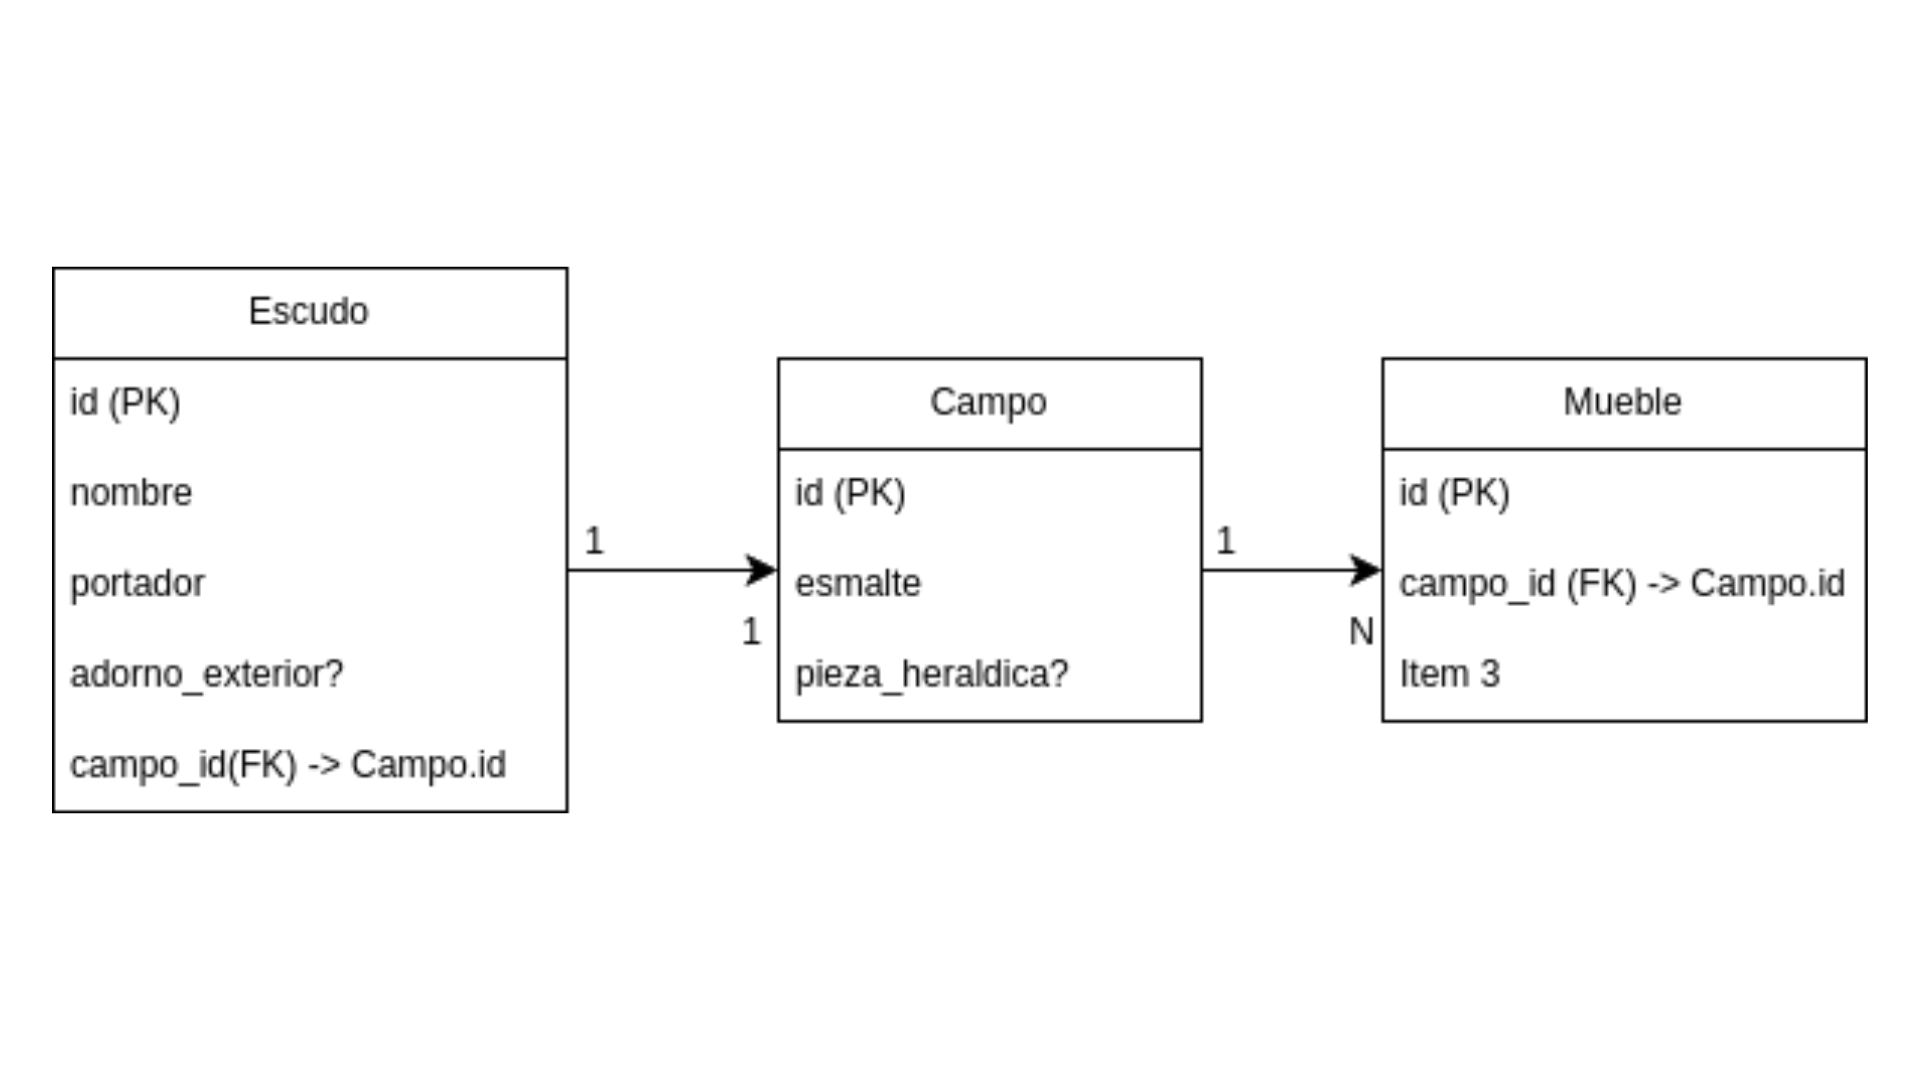
\includegraphics[width=0.7\textwidth]{figuras/diagramaBD.jpg}
    \caption{Relaciones entre las entidades del modelo de datos.}
    \label{fig:diagrama-bd}
\end{figure}

\subsection{Creación de la BD y prueba básica}
Tras definir el esquema se creó la base de datos SQLite y se verificó el guardado y la lectura de un escudo con un 
\emph{smoke test} mínimo. La prueba inserta un \texttt{Campo} (con esmalte), un mueble asociado y un \texttt{Escudo} que 
referencia ese campo; a continuación, recupera el escudo por \texttt{portador}. 

Para garantizar la repetibilidad y evitar dependencias entre ejecuciones, la prueba se ejecuta sobre una base de datos 
en memoria que se destruye automáticamente al finalizar. De este modo, se valida que las operaciones básicas de 
persistencia (creación, consulta y relación entre tablas) funcionan correctamente antes de continuar con la carga 
de datos reales.

\subsection{Carga del catálogo y compatibilidad con el modelo existente}
Una vez generada la base de datos y comprobada su persistencia, se integró la carga automática del catálogo a partir del 
archivo \texttt{JSON} existente. Esta funcionalidad permite mantener la compatibilidad con la estructura previa del sistema, 
de modo que el cambio de almacenamiento no afecta a las búsquedas ni a la interfaz actual.

La importación de datos se realiza mediante un script independiente `importar_json_db.py` que lee el catálogo en 
formato \texttt{JSON} y lo inserta en la base de datos de forma controlada. Este enfoque permite automatizar el proceso y 
mantener la reproducibilidad del entorno, garantizando que se pueda regenerar la base de datos a partir del mismo archivo de 
origen.

Durante la importación, los registros se insertan de manera idempotente, de manera que cada ejecución sustituye los datos 
existentes en lugar de duplicarlos. 

Se verificó en `test_carga_y_busqueda.py` que los datos se cargan correctamente y que las funcionalidades de filtrado 
siguen operativas. De este modo, el sistema puede seguir buscando por esmalte, portador, mueble, pieza heráldica o adorno 
exterior sin necesidad de modificar la lógica de negocio.

Hasta aquí, las búsquedas continúan ejecutándose en memoria tras recuperar los datos desde la base de datos, lo que resulta 
suficiente para un catálogo reducido y garantiza la compatibilidad con el código existente, pero conviene trasladar estas 
búsquedas directamente a la base de datos con el fin de mejorar el rendimiento y aprovechar el motor relacional para realizar 
consultas más eficientes sobre volúmenes de datos mayores.

Esta integración constituye el último paso para reemplazar completamente el almacenamiento en JSON por una base de datos 
relacional sin alterar la funcionalidad del catálogo.